%% abtex2-modelo-relatorio-tecnico.tex, v-1.9.7 laurocesar
%% Copyright 2012-2018 by abnTeX2 group at http://www.abntex.net.br/ 
%%
%% This work may be distributed and/or modified under the
%% conditions of the LaTeX Project Public License, either version 1.3
%% of this license or (at your option) any later version.
%% The latest version of this license is in
%%   http://www.latex-project.org/lppl.txt
%% and version 1.3 or later is part of all distributions of LaTeX
%% version 2005/12/01 or later.
%%
%% This work has the LPPL maintenance status `maintained'.
%% 
%% The Current Maintainer of this work is the abnTeX2 team, led
%% by Lauro César Araujo. Further information are available on 
%% http://www.abntex.net.br/
%%
%% This work consists of the files abntex2-modelo-relatorio-tecnico.tex,
%% abntex2-modelo-include-comandos and abntex2-modelo-references.bib
%%

% ------------------------------------------------------------------------
% ------------------------------------------------------------------------
% abnTeX2: Modelo de Relatório Técnico/Acadêmico em conformidade com 
% ABNT NBR 10719:2015 Informação e documentação - Relatório técnico e/ou
% científico - Apresentação
% ------------------------------------------------------------------------ 
% ------------------------------------------------------------------------

\documentclass[
	% -- opções da classe memoir --
	12pt,				% tamanho da fonte
	openright,			% capítulos começam em pág ímpar (insere página vazia caso preciso)
	twoside,			% para impressão em recto e verso. Oposto a oneside
	a4paper,			% tamanho do papel. 
	% -- opções da classe abntex2 --
	%chapter=TITLE,		% títulos de capítulos convertidos em letras maiúsculas
	%section=TITLE,		% títulos de seções convertidos em letras maiúsculas
	%subsection=TITLE,	% títulos de subseções convertidos em letras maiúsculas
	%subsubsection=TITLE,% títulos de subsubseções convertidos em letras maiúsculas
	% -- opções do pacote babel --
	english,			% idioma adicional para hifenização
	french,				% idioma adicional para hifenização
	spanish,			% idioma adicional para hifenização
	brazil,				% o último idioma é o principal do documento
	]{abntex2}


% ---
% PACOTES
% ---

% ---
% Pacotes fundamentais 
% ---
\usepackage{lmodern}			% Usa a fonte Latin Modern
\usepackage[T1]{fontenc}		% Selecao de codigos de fonte.
\usepackage[utf8]{inputenc}		% Codificacao do documento (conversão automática dos acentos)
\usepackage{indentfirst}		% Indenta o primeiro parágrafo de cada seção.
\usepackage{color}				% Controle das cores
\usepackage{graphicx}			% Inclusão de gráficos
\usepackage{microtype} 			% para melhorias de justificação
\usepackage{multirow}			% para mesclas linhas em tabelas
% ---

% ---
% Pacotes adicionais, usados no anexo do modelo de folha de identificação
% ---
\usepackage{multicol}
\usepackage{multirow}
% ---
	
% ---
% Pacotes adicionais, usados apenas no âmbito do Modelo Canônico do abnteX2
% ---
\usepackage{lipsum}				% para geração de dummy text
% ---

% ---
% Pacotes de citações
% ---
\usepackage[brazilian,hyperpageref]{backref}	 % Paginas com as citações na bibl
\usepackage[alf]{abntex2cite}	% Citações padrão ABNT

% --- 
% CONFIGURAÇÕES DE PACOTES
% --- 

% ---
% Configurações do pacote backref
% Usado sem a opção hyperpageref de backref
\renewcommand{\backrefpagesname}{Citado na(s) página(s):~}
% Texto padrão antes do número das páginas
\renewcommand{\backref}{}
% Define os textos da citação
\renewcommand*{\backrefalt}[4]{
	\ifcase #1 %
		Nenhuma citação no texto.%
	\or
		Citado na página #2.%
	\else
		Citado #1 vezes nas páginas #2.%
	\fi}%
% ---

% ---
% Informações de dados para CAPA e FOLHA DE ROSTO
% ---
\titulo{Documentação Técnica e Plano de Negócio \\ VisuMED}
\autor{Guilherme Souza da Silva \\ Jose Geraldo Fernandes Rabelo Filho \\ Marcelo Ferreira de Aquino}
\local{Brasil}
\data{2019}
\instituicao{%
  Universidade Federal do Amazonas
  \par
  Intituto de Computação}
\tipotrabalho{Relatório técnico}
% O preambulo deve conter o tipo do trabalho, o objetivo, 
% o nome da instituição e a área de concentração 
\preambulo{Plano de Negócio da empresa \textit{GMG Solutions} para o aplicativo \textit{VisuMED} a ser apresentado na disciplina de Sistemas Distribuidos no ano de 2019.}
% ---

% ---
% Configurações de aparência do PDF final

% alterando o aspecto da cor azul
\definecolor{blue}{RGB}{41,5,195}

% informações do PDF
\makeatletter
\hypersetup{
     	%pagebackref=true,
		pdftitle={\@title}, 
		pdfauthor={\@author},
    	pdfsubject={\imprimirpreambulo},
	    pdfcreator={LaTeX with abnTeX2},
		pdfkeywords={abnt}{latex}{abntex}{abntex2}{relatório técnico}, 
		colorlinks=true,       		% false: boxed links; true: colored links
    	linkcolor=blue,          	% color of internal links
    	citecolor=blue,        		% color of links to bibliography
    	filecolor=magenta,      		% color of file links
		urlcolor=blue,
		bookmarksdepth=4
}
\makeatother
% --- 

% --- 
% Espaçamentos entre linhas e parágrafos 
% --- 

% O tamanho do parágrafo é dado por:
\setlength{\parindent}{1.3cm}

% Controle do espaçamento entre um parágrafo e outro:
\setlength{\parskip}{0.2cm}  % tente também \onelineskip

% ---
% compila o indice
% ---
\makeindex
% ---

% ----
% Início do documento
% ----
\begin{document}

% Seleciona o idioma do documento (conforme pacotes do babel)
%\selectlanguage{english}
\selectlanguage{brazil}

% Retira espaço extra obsoleto entre as frases.
\frenchspacing 

% ----------------------------------------------------------
% ELEMENTOS PRÉ-TEXTUAIS
% ----------------------------------------------------------
% \pretextual

% ---
% Capa
% ---
\imprimircapa
% ---

% ---
% Folha de rosto
% (o * indica que haverá a ficha bibliográfica)
% ---
\imprimirfolhaderosto*
% ---

% resumo na língua vernácula (obrigatório)
\setlength{\absparsep}{18pt} % ajusta o espaçamento dos parágrafos do resumo
% ---


% inserir o sumario
% ---
\pdfbookmark[0]{\contentsname}{toc}
\tableofcontents*
\cleardoublepage
% ---

% ----------------------------------------------------------
% Parte de resultados
% ----------------------------------------------------------
\part{Documentação Técnica}

% ---
% Capitulo de revisão de literatura
% ---

\chapter{Resumo}

A importância do conhecimento, como fator de gerenciamento nas organizações, propicia um crescente interesse no entendimento das variáveis que impactam na implementação de recursos em empresas, organizações e países. Diante da relevância do assunto, a \textit{GMG Solutions} propõe uma ferramenta de visualização e análise de ocorrências relacionadas a saúde, chamada de \textit{VisuMED}. 

O objetivo do \textit{VisuMED} é  usar algoritmos coletores web de notícias que se aplicam a temas relacionados a saúde e que são importantes para gerenciamento de recursos, por exemplo, com a noticia \textit{"Homem leva facada nas costas após discussão e morre em hospital de Manaus"} o gestor responsável pelos hospitais da cidade pode aumentar ou diminuir o envio de determinado recurso ao hospital em questão.

O usuário (\textit{premium} ou \textit{não-premium}), através de seu dispositivo Android, terá acesso a uma lista de eventos ocorridos na cidade relacionados a saúde. Esses eventos serão marcados no mapa e poderão ser visualizados pelos usuário do aplicativo.

A método de alimentação das informações da plataforma será de maneira \textit{semi-colaborativa} através das redes sociais, ou seja, usará um algoritmo responsável pela coleta de publicações em redes sociais para alimentação de sua base de informação. Essas publicações serão interpretadas e adicionadas na lista de eventos de acordo com sua classificação.

A dinâmica de coleta de informação tem característica \textit{semi-colaborativa} pelo fato de ela ser produzida pelo usuário final, porém ela será coletada da rede social e não do usuário final.



\chapter{Brain-Storm Inicial}


A ideia dos desenvolvedores foi conciliadas por meio de um \textit{brainstorm} superficial, no qual conseguimos descrever tecnologias utilizadas e seus respectivos módulos, dividindo-se em \textit{frontend} e \textit{backend}.

\begin{center}
	\begin{tabular}{|l|l|l|}
		\hline
		\multicolumn{3}{|c|}{Tecnologias e Métodos} \\
		\hline
				 						& Tecnologias			& Módulos \\ \hline
		\multirow{3}{*}{FrontEnd} 		& RESTFul Web Service	& Disponibilizar os Metadados \\
										& IONIC 				& Exibir Relatórios\\
										& Google MAP API 		& Exibir Mapa\\ \hline
		\multirow{4}{*}{BackEnd}		& Crawler 				& Coletor de Dados na WEB\\
										& Scraper 				& Tratamento dos Dados \\
										& MongoDB 				& Armazenamento dos Dados \\
				 						& Python 				& Stemming \\ \hline
	\end{tabular}
\end{center}


\section*{RESTFul Web Service}

O Web Service irá disponibilizar os dados estruturados em JSON que posteriormente serão consumidos pelo app, desenvolvido em IONIC, para marcação dos eventos no mapa e geração de relatório.

\section*{IONIC}

O IONIC é um framework para desenvolvimento de aplicativos móveis híbridos criado em 2013, com ele teremos a possibilidade de desenvolver a aplicação multiplataforma. O IONIC  será usado para desenvolvimento da aplicação Mobile e WEB. 

\section*{Crawler}

Um rastreador da rede, em inglês \textit{web crawler}, é um programa de computador que navega pela internet de uma forma metódica e automatizada. Outros termos para rastreadores da rede são indexadores automáticos. A função do \textit{Crawler} no VisuMED será de coletar notícias de interesse do aplicativo para posteriormente ser salvo no Banco de Dados baseada em MongoDB.

\section*{Scraper}

Web scraping é uma técnica de extração de dados utilizada para coletar dados de sites por meio de processos automatizados. O Scraper faz extração de dados, da mesma forma, em uma cadeia de caracteres qualquer. A função do Scraper no VisuMED é categorizar as notícias indexadas pelo Crawler e determinar quais serão de interesse do aplicativo.

\section*{MongoDB}

MongoDB é um software de banco de dados não relacional orientado, de código aberto e multiplataforma, escrito na linguagem C++. Classificado como um programa de banco de dados NoSQL, o MongoDB usa documentos semelhantes a JSON com esquemas. O MongoDB será usado para armazenamento dos dados antes e depois do processamento feito pelo Scraper.


\chapter{Arquitetura}

\begin{figure}[h]
	\caption{\label{backend_figura}Arquitetura Back-End.}
	\begin{center}
		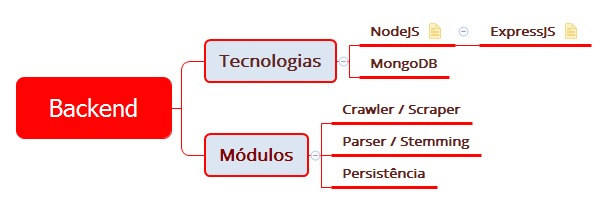
\includegraphics[scale=0.6]{figuras/arquitetura-backend.jpeg}
	\end{center}
\end{figure}


\begin{figure}[h]
	\caption{\label{frontend_figura}Arquitetura Front-End.}
	\begin{center}
		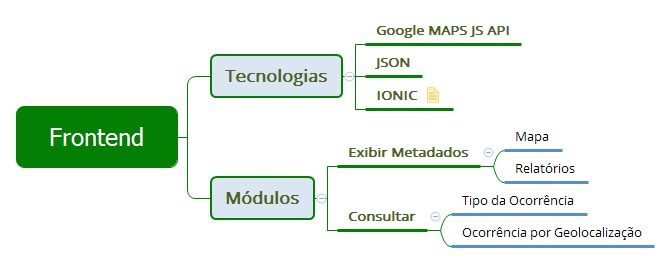
\includegraphics[scale=0.6]{figuras/arquitetura-frontend.jpeg}
	\end{center}
\end{figure}

\chapter{Mockups}

% ----------------------------------------------------------

\part{Plano de Negócio}

\chapter{Sumário Executivo}


\section{Resumo}

O plano negócio se resume em funcionalidades adicionais para usuários \textit{premium}. A funcionalidade disponível para usuários \textit{não-premium} será apenas visualização das ocorrência marcadas no mapa, enquanto usuários \textit{premium} terão dados  estatísticos e relatórios disponíveis de todas as localidade da cidade.

As pessoas beneficiadas pelo \textit{VisuMED} serão o público em geral, haja visto que o serviço prestado será de difusão de informações relacionadas a saúde. 

\textbf{O capital inicial da empresa veio dos sócios e o seu lucro e faturamento virá de contratos com órgãos públicos.}


\section{Dados dos empreendedores}

\begin{center}
	\begin{tabular}{|r|p{12cm}|}
		\hline
		\textbf{Nome:}		& Marcelo Ferreira de Aquino \\ \hline
		\textbf{Endereço:}	& Avenida Rodrigo Otávio. \\ \hline
		\textbf{Cidade:}	& Manaus \\ \hline
		\textbf{Estado:}	& Amazonas \\ \hline
		\textbf{Perfil:}	& Estudante de Engenharia da Computação na Universidade Federal do Amazonas\\ \hline
		\textbf{Atribuições:}	& Tratamento dos Dados (Scrapers) \\ \hline
	\end{tabular}
\end{center}

\begin{center}
	\begin{tabular}{|r|p{12cm}|}
		\hline
		\textbf{Nome:}		& Jose Geraldo Fernandes Rabelo Filho \\ \hline
		\textbf{Endereço:}	& Avenida Rodrigo Otávio. \\ \hline
		\textbf{Cidade:}	& Manaus \\ \hline
		\textbf{Estado:}	& Amazonas \\ \hline
		\textbf{Perfil:}	& Estudante de Engenharia da Computação na Universidade Federal do Amazonas\\ \hline
		\textbf{Atribuições:}	& Desenvolvimento do Ambiente (IONIC) \\ \hline
	\end{tabular}
\end{center}

\begin{center}
	\begin{tabular}{|r|p{12cm}|}
		\hline
		\textbf{Nome:}		& Guilherme Souza da Silva \\ \hline
		\textbf{Endereço:}	& Avenida Rodrigo Otávio. \\ \hline
		\textbf{Cidade:}	& Manaus \\ \hline
		\textbf{Estado:}	& Amazonas \\ \hline
		\textbf{Perfil:}	& Estudante de Engenharia da Computação na Universidade Federal do Amazonas\\ \hline
		\textbf{Atribuições:}	& Coleta dos dados (Crawlers) \\ \hline
	\end{tabular}
\end{center}

\begin{center}
	\begin{tabular}{|r|p{12cm}|}
		\hline
		\textbf{Nome:}		& Eduardo James Souto \\ \hline
		\textbf{Endereço:}	& Avenida Rodrigo Otávio. \\ \hline
		\textbf{Cidade:}	& Manaus \\ \hline
		\textbf{Estado:}	& Amazonas \\ \hline
		\textbf{Perfil:}	& Professor na Universidade Federal do Amazonas \\ \hline
		\textbf{Atribuições:}	& Investidor \\ \hline
	\end{tabular}
\end{center}

\section{Missão da Empresa}

Levar informações relacionadas a saúde ao público em geral, além de realizar análise estatísticas relacionadas ao eventos indexados pelo aplicativo e direcioná-los as regiões da cidade de Manaus-AM.

\section{Setor de Atividade}

[ ] Agropecuária

[ ] Comércio

[ ] Indústria

[X] Serviços

\section{Forma Jurídica}

( ) Empresário Individual

( ) Empresa Individual de Responsabilidade Limitada – EIRELI

( ) Microempreendedor Individual – MEI

(x) Sociedade Limitada

( ) Outros:

\section{Capital Social}

\begin{center}
	\begin{tabular}{|c|c|c|c|}
		\hline
		\textbf{No:}	& \textbf{Sócio}				& \textbf{Valor} & \textbf{Participação} \\ \hline
		1				& Marcelo Ferreira de Aquino 	& R\$ 48,99 & 16,33\% \\ \hline
		2				& José Geraldo Rabelo 			& R\$ 48,99 & 16,33\% \\ \hline
		3				& Guilherme de Souza 			& R\$ 48,99 & 16,33\% \\ \hline
		4				& Eduardo Souto 				& R\$ 153,03 & 51,01\% \\ \hline
		\textbf{Total}	& 	 							& \textbf{R\$ 300,00} & \textbf{100\% }\\ \hline
	\end{tabular}
\end{center}

\section{Fonte do Recurso}

A abertura da empresa se deu através de investimento de capital próprio dos sócios.


%--------------------------------------------------

\chapter{Análise de Mercado}

\section{Estudo dos Clientes}

\subsection{Público Alvo}

\begin{itemize}
	\item Agentes públicos e privados do sistema de saúde
	\item Imobiliárias
	\item Agentes de Segurança
	\item Seguradoras
\end{itemize}

\subsection{Comportamento dos clientes (interesses e o que os levam a comprar)}


\subsection{Área de abrangência (onde estão os clientes?)}

\section{Estudo dos Concorrentes}

\begin{itemize}
	\item IPEA 
		\subitem \textbf{Qualidade:} 
		\subitem \textbf{Preço:} 
		\subitem \textbf{Condições de Pagamento:} 
		\subitem \textbf{Qualidade:} 
		\subitem \textbf{Atendimento:} 
		\subitem \textbf{Serviço aos Clientes:} 

	\item PRODAM 
		\subitem \textbf{Qualidade:} 
		\subitem \textbf{Preço:} 
		\subitem \textbf{Condições de Pagamento:} 
		\subitem \textbf{Qualidade:} 
		\subitem \textbf{Atendimento:} 
		\subitem \textbf{Serviço aos Clientes:} 
		 
\end{itemize}

\subsection*{Conclusões}


%------------------------------------------------

\chapter{Plano de Marketing}

\section{Produtos e Serviços}

\section{Preços}

\section{Estratégias promocionais}

\section{Estrutura de comercialização}

\section{Localização do negócio}

\begin{center}
	\begin{tabular}{|r|p{12cm}|}
		\hline
		\textbf{Endereço:}	& Av. General Rodrigo Otávio \\ \hline
		\textbf{Bairro:}	& Coroado I. \\ \hline
		\textbf{Cidade:}	& Manaus \\ \hline
		\textbf{Estado:}	& Amazonas \\ \hline
		\textbf{Telefone:}	&  \\ \hline
	\end{tabular}
\end{center}


%---------------------------------------------------

\chapter{Plano Operacional}

\section{Capacidade Instalada}

\section{Processos Operacionais}

\section{Necessidade Pessoal}


%--------------------------------------------------

\chapter{Plano Financeiro}

\section{Investimento total}


%--------------------------------------------------

\chapter{Conclusão}

\section{Investimento total}

	


% ----------------------------------------------------------
% Anexos
% ----------------------------------------------------------

% ---
% Inicia os anexos
% ---
\begin{anexosenv}

% Imprime uma página indicando o início dos anexos
\partanexos

% ---
\chapter{Morbi ultrices rutrum lorem.}
% ---
\lipsum[30]


\end{anexosenv}

%---------------------------------------------------------------------
% INDICE REMISSIVO
%---------------------------------------------------------------------

\phantompart

\printindex

%---------------------------------------------------------------------
% Formulário de Identificação (opcional)
%---------------------------------------------------------------------
\chapter*[Formulário de Identificação]{Formulário de Identificação}
\addcontentsline{toc}{chapter}{Exemplo de Formulário de Identificação}
\label{formulado-identificacao}

Exemplo de Formulário de Identificação, compatível com o Anexo A (informativo)
da ABNT NBR 10719:2015. Este formulário não é um anexo. Conforme definido na
norma, ele é o último elemento pós-textual e opcional do relatório.

\bigskip

\begin{tabular}{|p{9cm}|p{5cm}|}
\hline
\multicolumn{2}{|c|}{\textbf{\large Dados do Relatório Técnico e/ou científico}}\\
\hline
\multirow{4}{10cm}[24pt]{Título e subtítulo}& Classificação de segurança\\
                   & \\
                   \cline{2-2}
                   & No.\\
                   & \\
				
\hline
Tipo de relatório & Data\\
\hline
Título do projeto/programa/plano & No.\\
\hline
\multicolumn{2}{|l|}{Autor(es)} \\
\hline
\multicolumn{2}{|l|}{Instituição executora e endereço completo} \\
\hline
\multicolumn{2}{|l|}{Instituição patrocinadora e endereço completo} \\
\hline
\multicolumn{2}{|l|}{Resumo}\\[3cm]
\hline
\multicolumn{2}{|l|}{Palavras-chave/descritores}\\
\hline
\multicolumn{2}{|l|}{
Edição \hfill No. de páginas \hfill No. do volume \hfill Nº de classificação \phantom{XXXX}} \\
\hline
\multicolumn{2}{|l|}{
ISSN \hfill \hfill Tiragem \hfill Preço \phantom{XXXXXXXX}} \\
\hline
\multicolumn{2}{|l|}{Distribuidor} \\
\hline
\multicolumn{2}{|l|}{Observações/notas}\\[3cm]
\hline
\end{tabular}

\end{document}
